        \clearpage
        \begin{figure*}[ht]
            \pdfbookmark[2]{ID 05}{figure_id_05}
        	\centering
            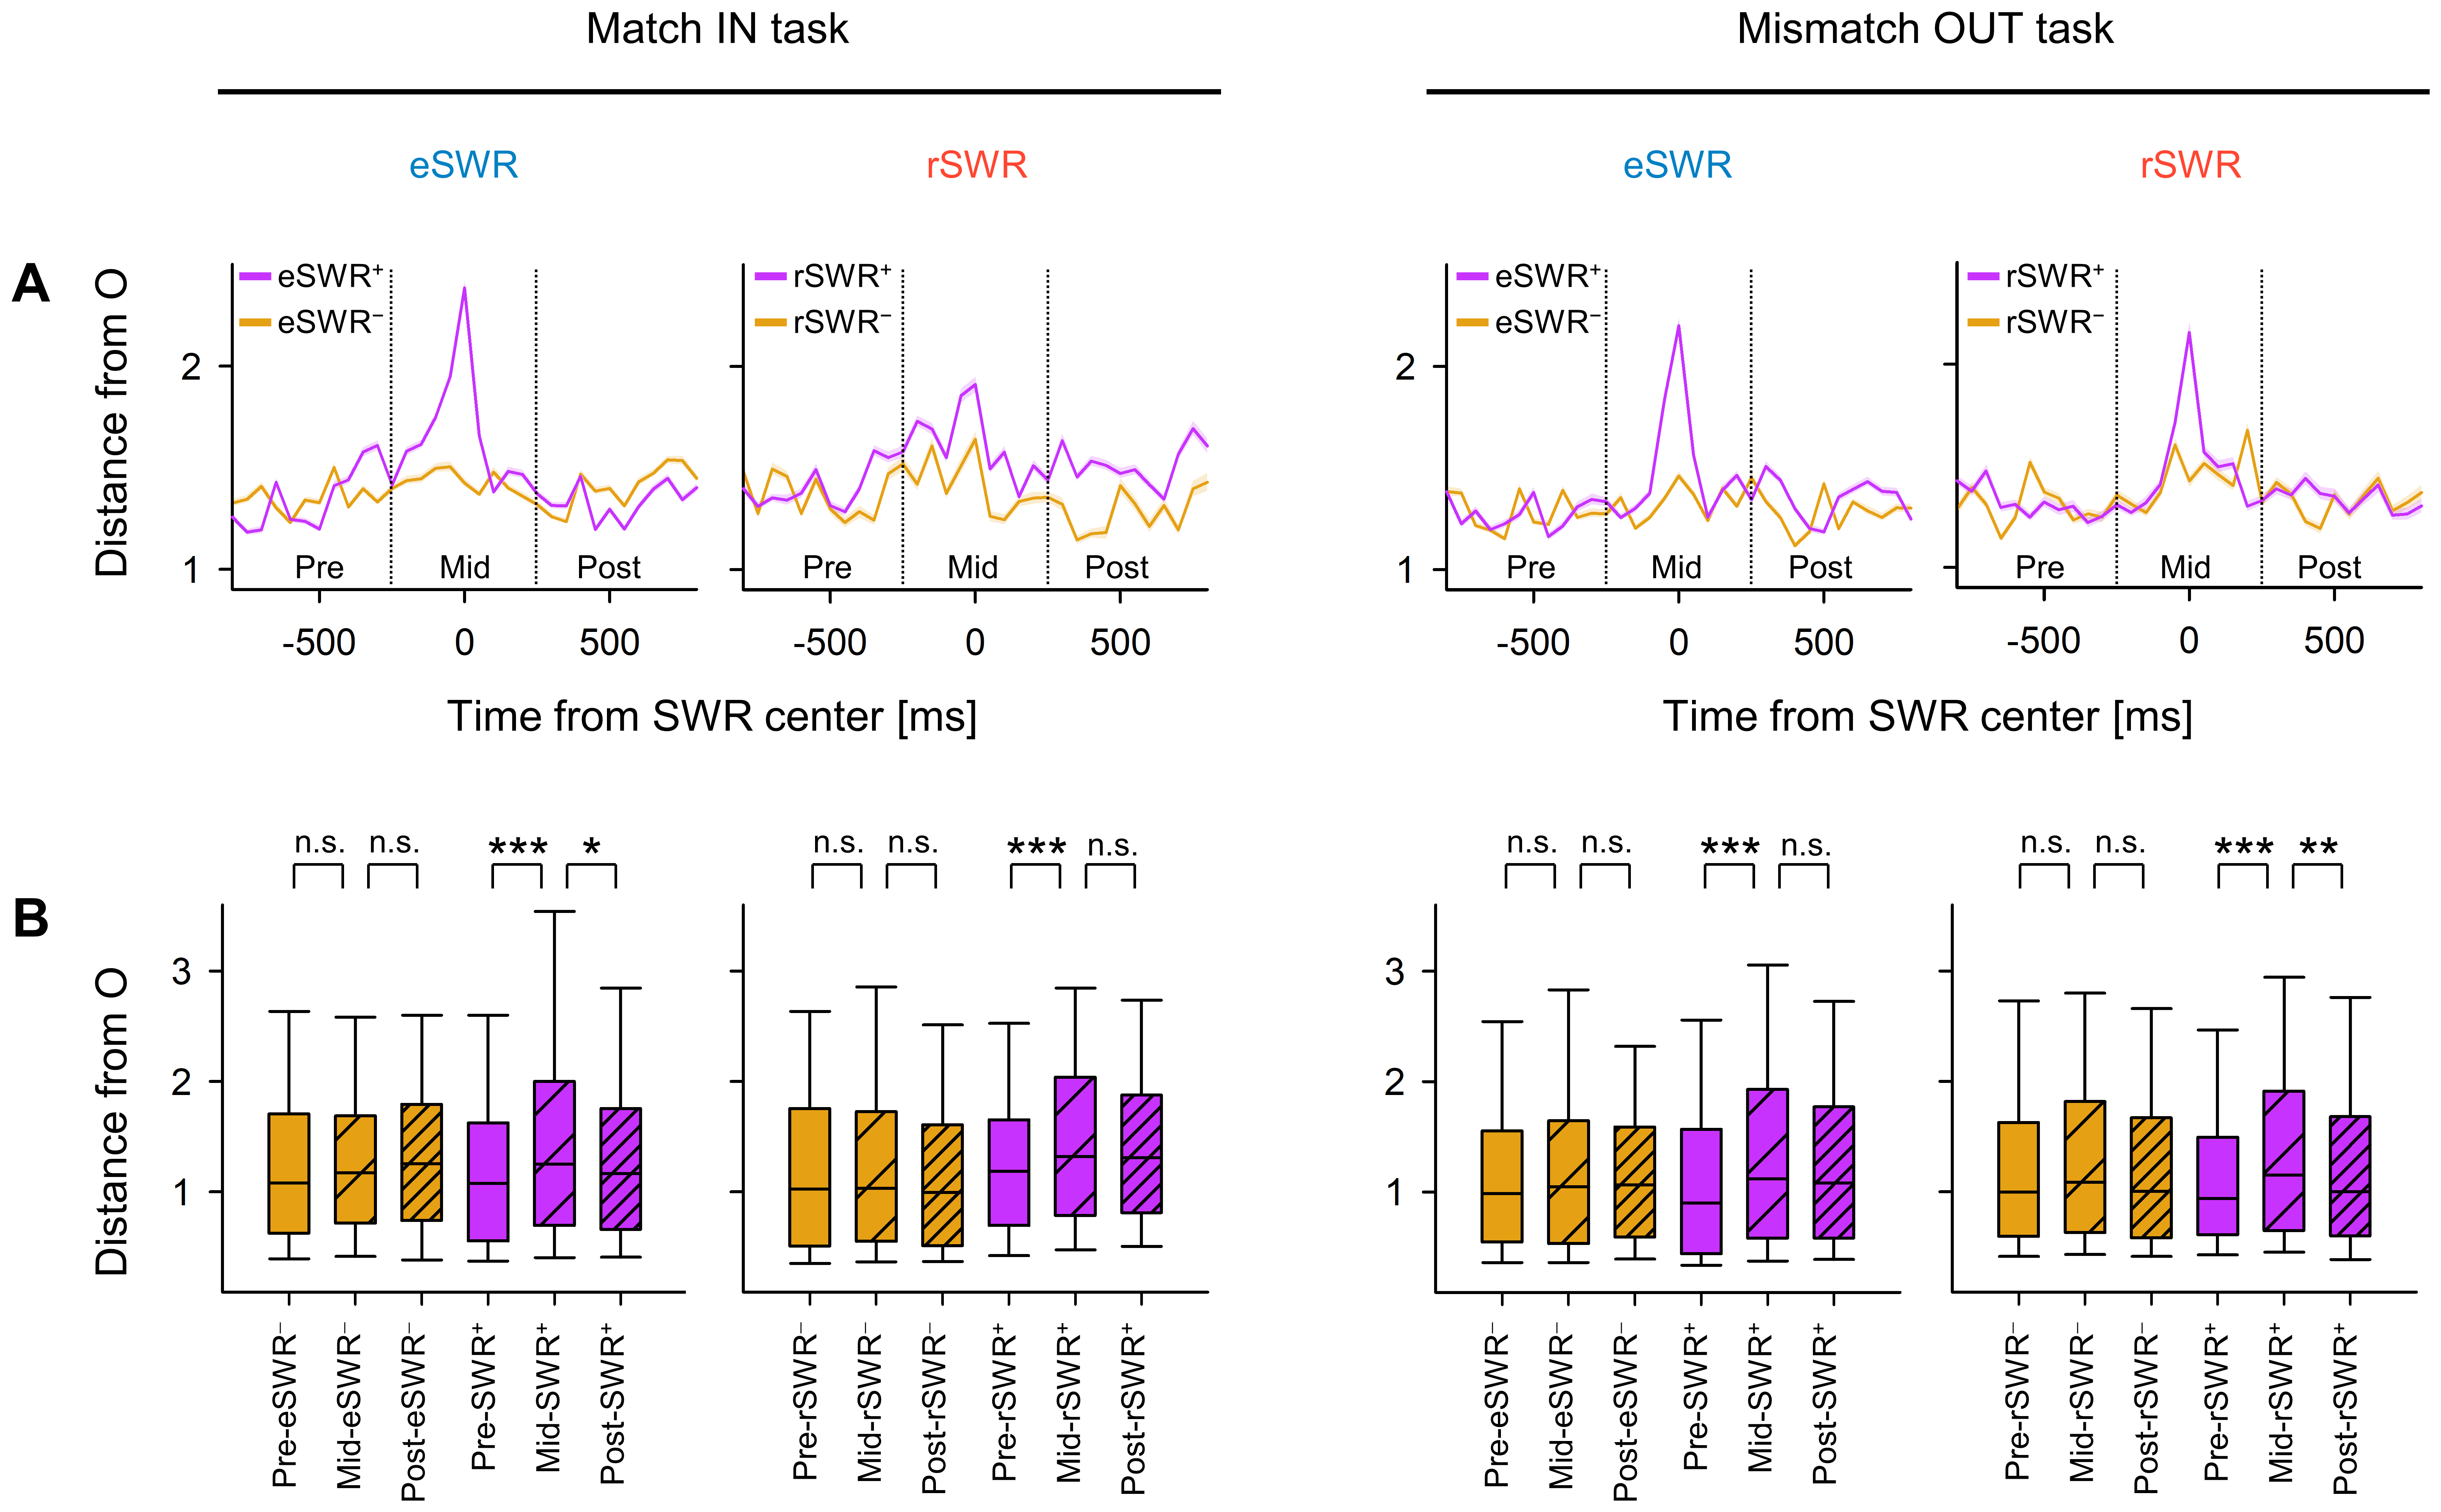
\includegraphics[width=1\textwidth]{./src/figures/.png/Figure_ID_05.png}
        	\caption{\textbf{
Transient neural trajectory change during SWR
}
\smallskip
\\
\textbf{\textit{A.}} Distance from the origin ($O$) of the peri-sharp-wave-ripple trajectory (mean \textpm 95\% confidence interval, although the intervals might not be visible due to their narrow ranges. \textbf{\textit{B.}}  The distance from the origin ($O$) during pre-, mid-, and post-SWR periods (*\textit{p} $<$ 0.05, **\textit{p} $<$ 0.01, ***\textit{p} $<$ 0.001; Brunner--Munzel test). Abbreviations: SWR, sharp-wave ripple events; eSWR, SWR during the encoding phase; rSWR, SWR during the retrieval phase, SWR$^+$, SWR event; SWR$^-$ control events for SWR$^+$; pre-, mid-, or post-SWR, the time interval from $-800$ to $-250$ ms, from $-250$ to $+250$ ms, or from $+250$ to $+800$ ms relative to SWR center.
}
% width=1\textwidth
        	\label{fig:05}
        \end{figure*}
